\documentclass[10pt,a4paper,oneside]{article}
\usepackage[utf8]{inputenc}
\usepackage[T1]{fontenc}
\usepackage{amsmath}
\usepackage{amsfonts}
\usepackage{amssymb}
\usepackage{enumerate}
\usepackage{graphicx}
\usepackage{framed}
\usepackage{tikz} %%% VIP %%%
\begin{document}
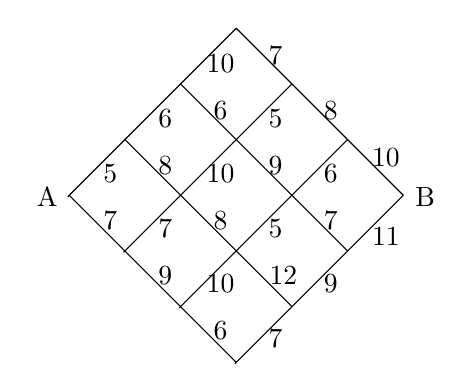
\begin{tikzpicture}
\draw(0,0) grid [rotate=45](3,3)
node at (-2.4,2.1) {A} 
node at (-1.6,1.8) {7}
node at (-1.6,2.4){5}
node at (-0.9,2.5){8}
node at (-0.9,3.1){6}
node at (-0.9,1.7){7}
node at (-0.9,1.1){9}
node at (-0.2,1 ){10}
node at (-0.2,0.4){6}
node at (-0.2,2.4){10}
node at (-0.2,1.8){8}
node at (-0.2,3.2){6}
node at (-0.2,3.8){10}
node at (0.5,0.3){7}
node at (0.6,1.1){12}
node at (0.5,1.7){5}
node at (0.5,2.5){9}
node at (0.5,3.1){5}
node at (0.5,3.9){7}
node at (1.2,1){9}
node at (1.2,1.8){7}
node at (1.2,2.4){6}
node at (1.2,3.2){8}
node at (1.9,1.6){11}
node at (1.9,2.6){10}
node at (2.4,2.1){B};
\end{tikzpicture}
\\
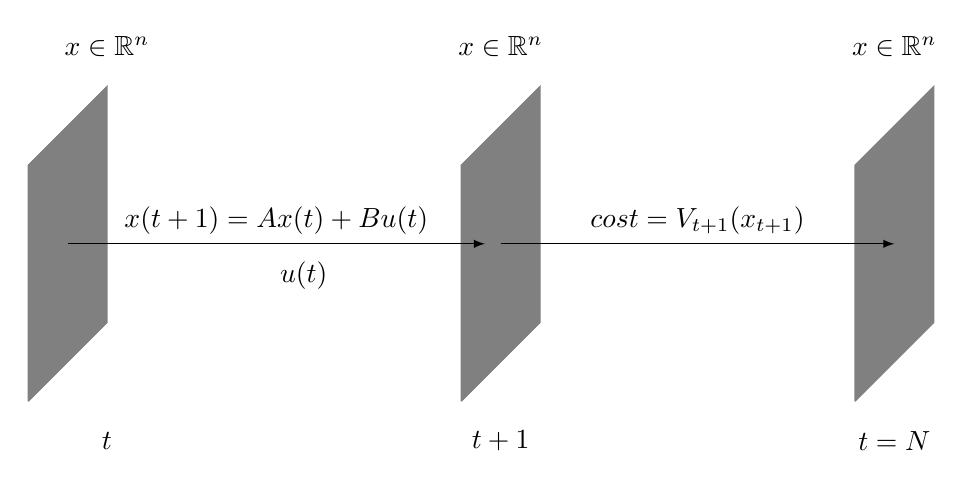
\begin{tikzpicture}[auto,>=latex]
\filldraw[gray] (-0.5,0)--(-0.5,3)--(0.5,4)--(0.5,1)--(-0.5,0);
\filldraw[gray] (5,0)--(5,3)--(6,4)--(6,1)--(5,0);
\filldraw[gray] (10,0)--(10,3)--(11,4)--(11,1)--(10,0);
\draw node at (0.5,-0.5) {$t$};
\draw node at (5.5,-0.5) {$t+1$};
\draw node at (10.5,-0.5) {$t=N$};
\draw node at (0.5,4.5) {$x\in\mathbb{R}^n$};
\draw node at (5.5,4.5) {$x\in\mathbb{R}^n$};
\draw node at (10.5,4.5) {$x\in\mathbb{R}^n$};
\draw node at (3, 1.6) {$u(t)$};
\draw[->](0,2)-- node {$x(t+1)=Ax(t)+Bu(t)$}(5.3,2);
\draw[->](5.5,2)-- node {$cost=V_{t+1}(x_{t+1})$}(10.5,2);
\end{tikzpicture}
\end{document}